\documentclass{article}

\title{Complex Variables Homework Section 4}
\author{Adam Buskirk}

\usepackage{amssymb,amsmath,amsthm}
\usepackage{tikz}
\usepackage[margin=1in]{geometry}

\newtheorem{theorem}[subsection]{Theorem}
\newtheorem{conjecture}[subsection]{Conjecture}
\newtheorem{lemma}[subsection]{Lemma}
\theoremstyle{definition}
\newtheorem{definition}[subsection]{Definition}

\newcommand{\R}{\mathbb{R}}
\newcommand{\N}{\mathbb{N}}
\newcommand{\Q}{\mathbb{Q}}
\newcommand{\Z}{\mathbb{Z}}
\newcommand{\p}[1]{\left(#1\right)}
\newcommand{\set}[1]{\left\{#1\right\}}
% \newcommand{\p}[1]{\left(#1\right)}

\begin{document}
\maketitle

Sec.\ 4, problem \#5.

\section*{Problem 4.5}
\begin{figure}[h]
\centering
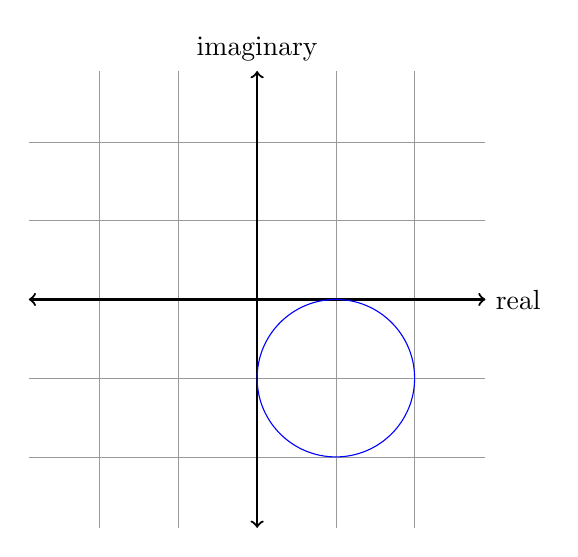
\begin{tikzpicture}[domain=-2:2]
\draw[very thin,color=black!40] (-2.9,-2.9) grid (2.9,2.9);
\draw[thick,<->] (-2.9,0) -- (2.9,0) node[right] {real};
\draw[thick,<->] (0,-2.9) -- (0,2.9) node[above] {imaginary};
\draw[color=blue] (1,-1) circle (1);
\end{tikzpicture}
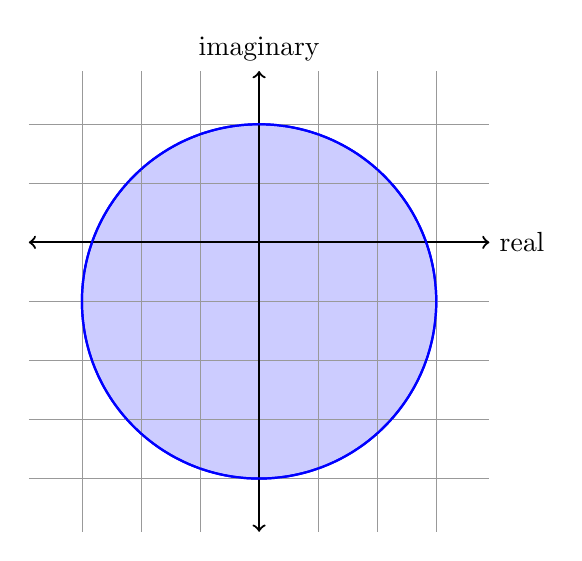
\begin{tikzpicture}[scale=0.75,domain=-4:4]
\draw[thick,color=blue,fill=blue!20] (0,-1) circle (3);
\draw[very thin,color=black!40] (-3.9,-4.9) grid (3.9,2.9);
\draw[thick,<->] (-3.9,0) -- (3.9,0) node[right] {real};
\draw[thick,<->] (0,-4.9) -- (0,2.9) node[above] {imaginary};
\draw[thick,color=blue] (0,-1) circle (3);
\end{tikzpicture}
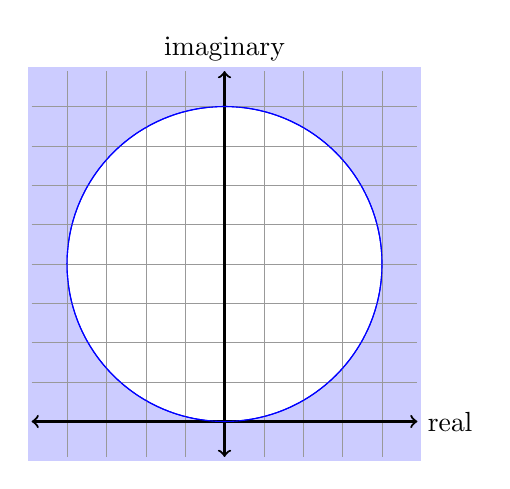
\begin{tikzpicture}[scale=0.5,domain=-4:4]
\fill[blue!20] (-5,-1) -- (-5,9) -- (5,9) -- (5,-1) -- cycle;
\draw[color=blue,fill=white] (0,4) circle (4);
\draw[very thin,color=black!40] (-4.9,-0.9) grid (4.9,8.9);
\draw[thick,<->] (-4.9,0) -- (4.9,0) node[right] {real};
\draw[thick,<->] (0,-0.9) -- (0,8.9) node[above] {imaginary};
\draw[color=blue] (0,4) circle (4);
\end{tikzpicture}
\caption{The answers to part a (upper left), part b (upper right), and part c (bottom) 
respectively.}
\end{figure}
\end{document}
